\pdfminorversion=4
\documentclass[a4paper,12pt]{article}

%%%%%%%%%%%%%%%%%%%
% Packages/Macros %
%%%%%%%%%%%%%%%%%%%
\usepackage{amssymb,latexsym,amsmath}     % Standard packages
\usepackage[utf8]{inputenc}
\usepackage[portuguese]{babel}
\usepackage[T1]{fontenc}
\usepackage{titlesec}
\usepackage{blindtext}
\usepackage{graphicx}
\usepackage{indentfirst}
\usepackage[a4paper, margin=1in]{geometry}

%%%%%%%%%%%
% Margins %
%%%%%%%%%%%
\addtolength{\textwidth}{1.0in}
\addtolength{\textheight}{1.00in}
\addtolength{\evensidemargin}{-0.5in}
\addtolength{\oddsidemargin}{-0.5in}
\addtolength{\topmargin}{-.50in}


%%%%%%%%%%%%%%%%%%%%%%%%%%%%%%
% Theorem/Proof Environments %
%%%%%%%%%%%%%%%%%%%%%%%%%%%%%%
\newtheorem{theorem}{Theorem}
\newenvironment{proof}{\noindent{\bf Proof:}}{$\hfill \Box$ \vspace{10pt}}  


%%%%%%%%%%%%%%%%%%%%%%%%%%%%%%%%%%%%%%%%%%%%%%%%%%%%%%%%%%%%%%%%%%%%%%%%
% 
%                               DOCUMENT                              
%
%%%%%%%%%%%%%%%%%%%%%%%%%%%%%%%%%%%%%%%%%%%%%%%%%%%%%%%%%%%%%%%%%%%%%%%%

\begin{document}

\title{ROTEIRO-07-FSC326-2018-2\_VRS\_ALUNO   \hbox{Carga e Descarga de Capacitores - Circuito-RC/DC} } 

%\title{Sample \LaTeX ~File}
\author{Zimermann, H. R.}
\date{Versão: \today{}}
\maketitle

\begin{abstract}
Este roteiro tem objetivo de guiar as atividades de estudo (leitura, exercícios e experimentos). As atividades que serão usadas para avaliação serão disponibilizadas no \hbox{portalfisica.com/fsc326.html} e também no AVEA Moodle UFSM \hbox{http://ead06.proj.ufsm.br} na área da disciplina de Laboratório de Física III no decorrer do período dessas atividades.
\end{abstract}

\hrule{}

\section{Objetivo}

Verificar como variam a corrente e a carga durante a descarga de um capacitor. 

\section{Fundamentos das medidas }
 
Os circuitos de corrente contínua (DC) apresentam uma característica importante, a saber, a corrente que flui nesse circuito é esperada que seja constante (estável) e que possa fluir em qualquer sentido no circuito. Uma peculiaridade dos circuitos DC é quando nesse circuito um componente capacitivo (Capacitor) é adicionado, então embora a corrente elétrica flua (após estabelecida) apenas em um sentido ela pode variar no tempo. Circuitos de contém um componente resistivo (Resistor) e um capacitivo (Capacitor) associados em série, são chamados de \textbf{Circuitos RC}.

 
\section*{Carga do Capacitor} 

\vspace{.5ex}

Para analisar quantitativamente um circuito RC simples, aplica-se a regra da malhas de Kirchhoff [1]. Tomando como exemplo o percurso da malha na Figura \ref{fig:1}\textit{b} no sentido horário:

\begin{equation} \label{eq:1}
\varepsilon - \frac{q}{C}-IR=0    
\end{equation}


em que $\varepsilon$ representa a força eletromotriz (\textit{fem}), ou seja a diferença de potencial (\textbf{ddp}) da fonte, $q/C$ é a diferença de potencial no capacitor e $IR$ é a diferença de potencial no resistor. Para a convenção de sinais se utiliza a descrita no \textbf{(Anexo \ref{anx:a})} para os sinais em $\varepsilon$ e $IR$. O capacitor é percorrido, pela corrente elétrica, na direção da placa positiva para a negativa, o que representa um decréscimo no potencial. Portanto, utilizamos um sinal negativo para essa diferença potencial na Equação \ref{eq:1}. Note que $q$ e $I$ são valores "instantâneos" que dependem do tempo (em oposição aos valores de estado estacionários) conforme o capacitor estiver sendo carregado. 

\begin{figure}[htp]
\centering
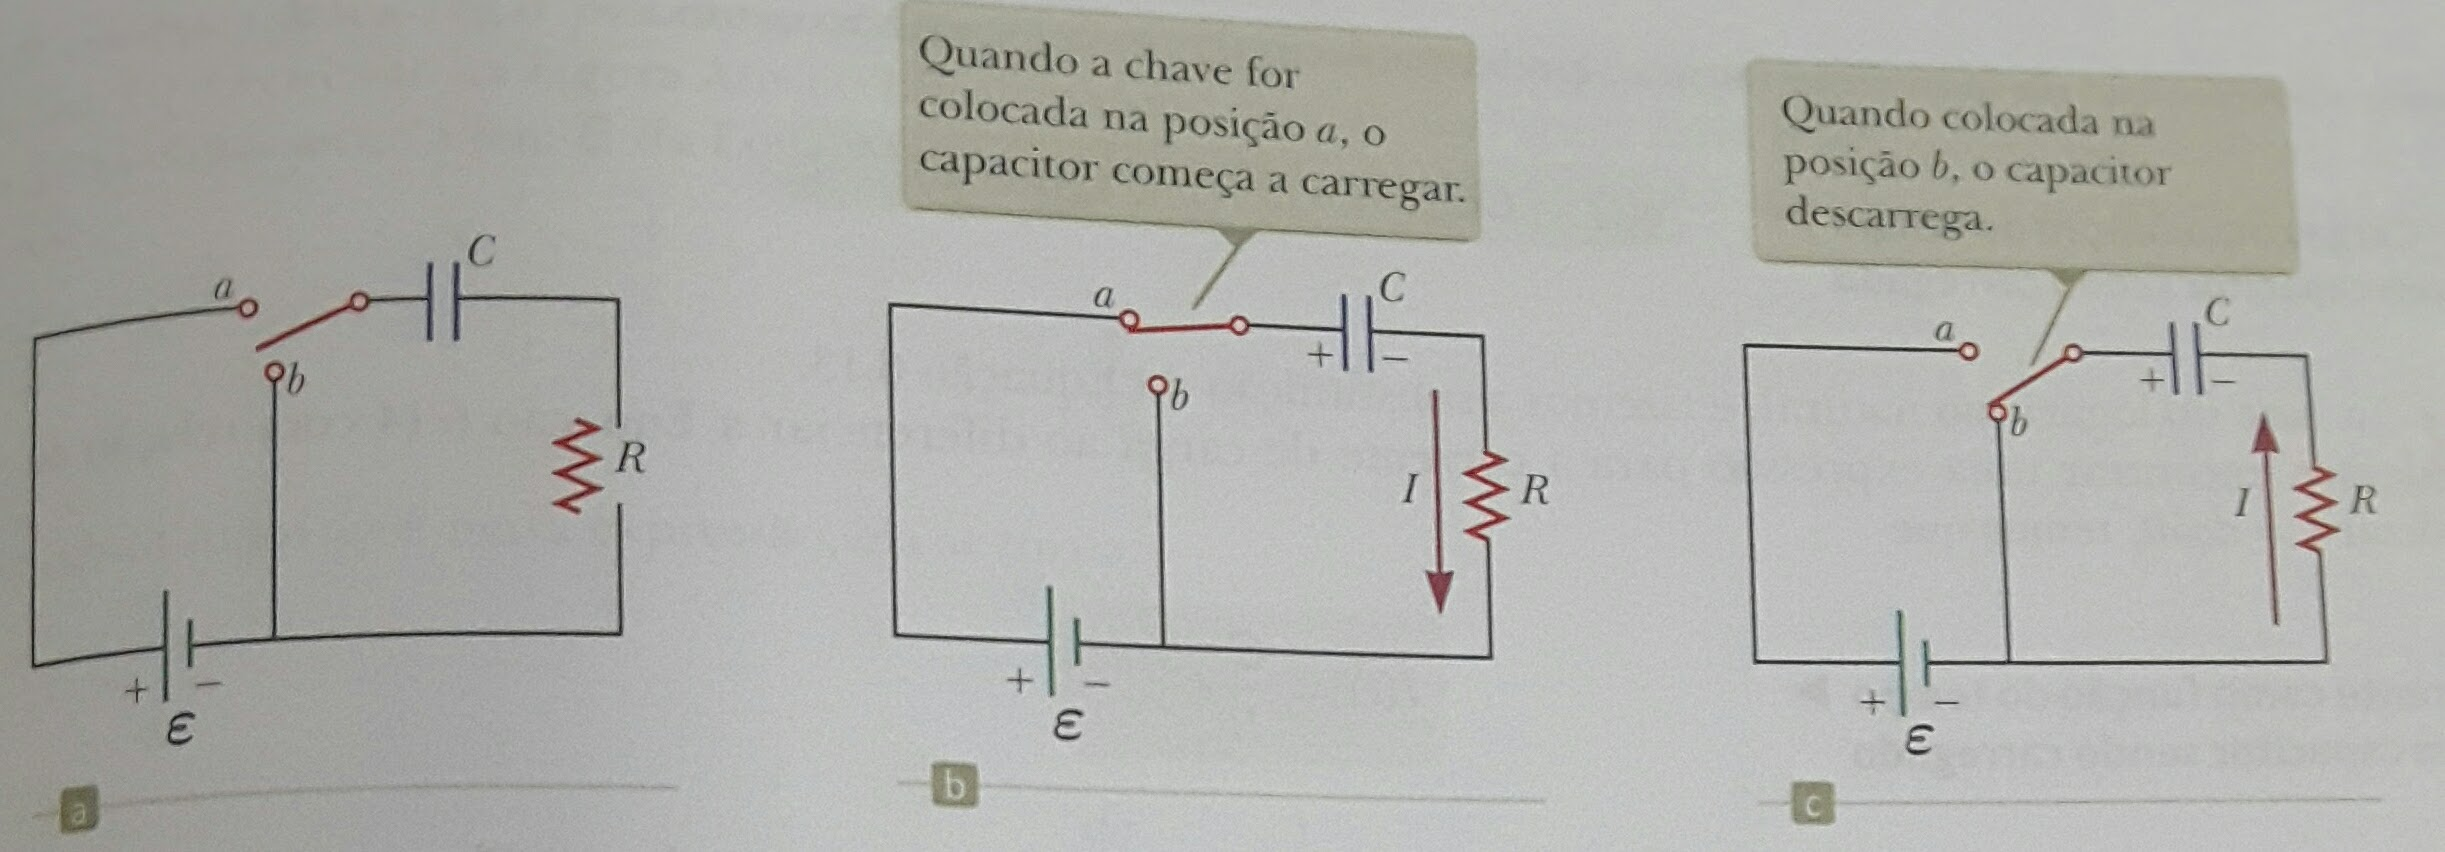
\includegraphics[width=14.5cm]{fig1}
\caption{Capacitor em série com um resistor, chave e bateria. \textit{Fonte: Jewett, JR Serway (2011)\cite{jeewett11}}}
\label{fig:1}
\end{figure}

Podemos utilizar a Equação \ref{eq:1} para encontrar a corrente inicial no circuito e na carga máxima no capacitor. No momento em que a chave é colocada na posição $a\;(t=0)$, a carga no capacitor é \textit{zero}. A Equação \ref{eq:1} mostra que a corrente inicial $I_i$ no circuito é máxima, dada por

\begin{equation} \label{eq:2}
I_i = \frac{\varepsilon}{R} \; \;(\textbf{corrente em } t=0)
\end{equation}

Nessa hora, a diferença potencial dos terminais da bateria aparece completamente no resistor. Mais tarde, o capacitor é carregado no seu valor máximo $Q$, a carga deixa de fluir, a corrente no circuito é \textit{zero} e a diferença potencial dos terminais da bateria aparece completamente no capacitor. A substituição de $I=0$ na Equação \ref{eq:1} dá a carga máxima no capacitor:

\begin{equation} \label{eq:3}
Q = C\varepsilon \;\; (\textbf{carga máxima})
\end{equation}

Para determinar expressões analíticas para a dependência do tempo da carga e corrente, devemos resolver a Equação \ref{eq:1}, uma única equação com duas variáveis $q$ e $I$. A corrente em todas as partes do circuito em série deve ser a mesma. Portante, a corrente na resistência $R$ deve ser a mesma que aquela entre cada placa de capacitor e o fio conectado a ele. Essa corrente é igual à taxa de variação no tempo da carga nas placas do capacitor. Assim, substituímos $I= dq/dt$ na Equação \ref{eq:1} e a reposicionamos:


$$
\frac{dq}{dt} = \frac{\varepsilon}{R} - \frac{q}{RC}
$$

Para encontrar uma expressão para $q$ resolvemos essa equação diferencial separável como segue. Primeiro, combine os termos do lado direito:

$$
\frac{dq}{dt} = \frac{C\varepsilon}{RC} - \frac{q}{RC} = - \frac{ q-C\varepsilon}{RC}
$$

Multiplique essa equação por $dt$ e divida por $q-C\varepsilon$:

$$
\frac{dq}{q-C\varepsilon} = - \frac{1}{RC}dt
$$

Integre essa expressão, utilizando $q=0$ em $t=0$:

\begin{gather*} 
\int_{0}^{q} \frac{dq}{q-C\varepsilon} = -\frac{1}{RC}\int_{0}^{t}dt \\ 
 ln \left( \frac{q-C\varepsilon}{-C\varepsilon} \right) = - \frac{t}{RC}
\end{gather*}

A partir da definição do logaritmo natural, podemos formular essa expressão como

$$
q=C\varepsilon(1-e^{-t/RC})
$$
\begin{equation} \label{eq:4}
q(t)= Q(1-e^{-t/RC})\;(\textbf{carga do capacitor})
\end{equation}

onde $e$ é a base do logaritmo natural, e fizemos a substituição da Equação \ref{eq:3}, essa equação pode ser entendida como (\textbf{Carga como função do tempo para um capacitor sendo carregado})

Podemos encontrar uma expressão para a corrente de carga ao diferenciar a Equação \ref{eq:4} com relação ao tempo. Ao utilizar $I=dq/dt$, temos que

\begin{equation} \label{eq:5}
I(t) = \frac{\varepsilon}{R}e^{-t/RC}\;(\textbf{corrente de carga do capacitor})
\end{equation}

A expressão acima pode ser entendida como: \textbf{Corrente como função do tempo para um capacitor carregando}.
Representações da carga de capacitor e corrente de circuito por tempo são mostradas na Figura \ref{fig:2}. 

\begin{figure}[htp]
\centering
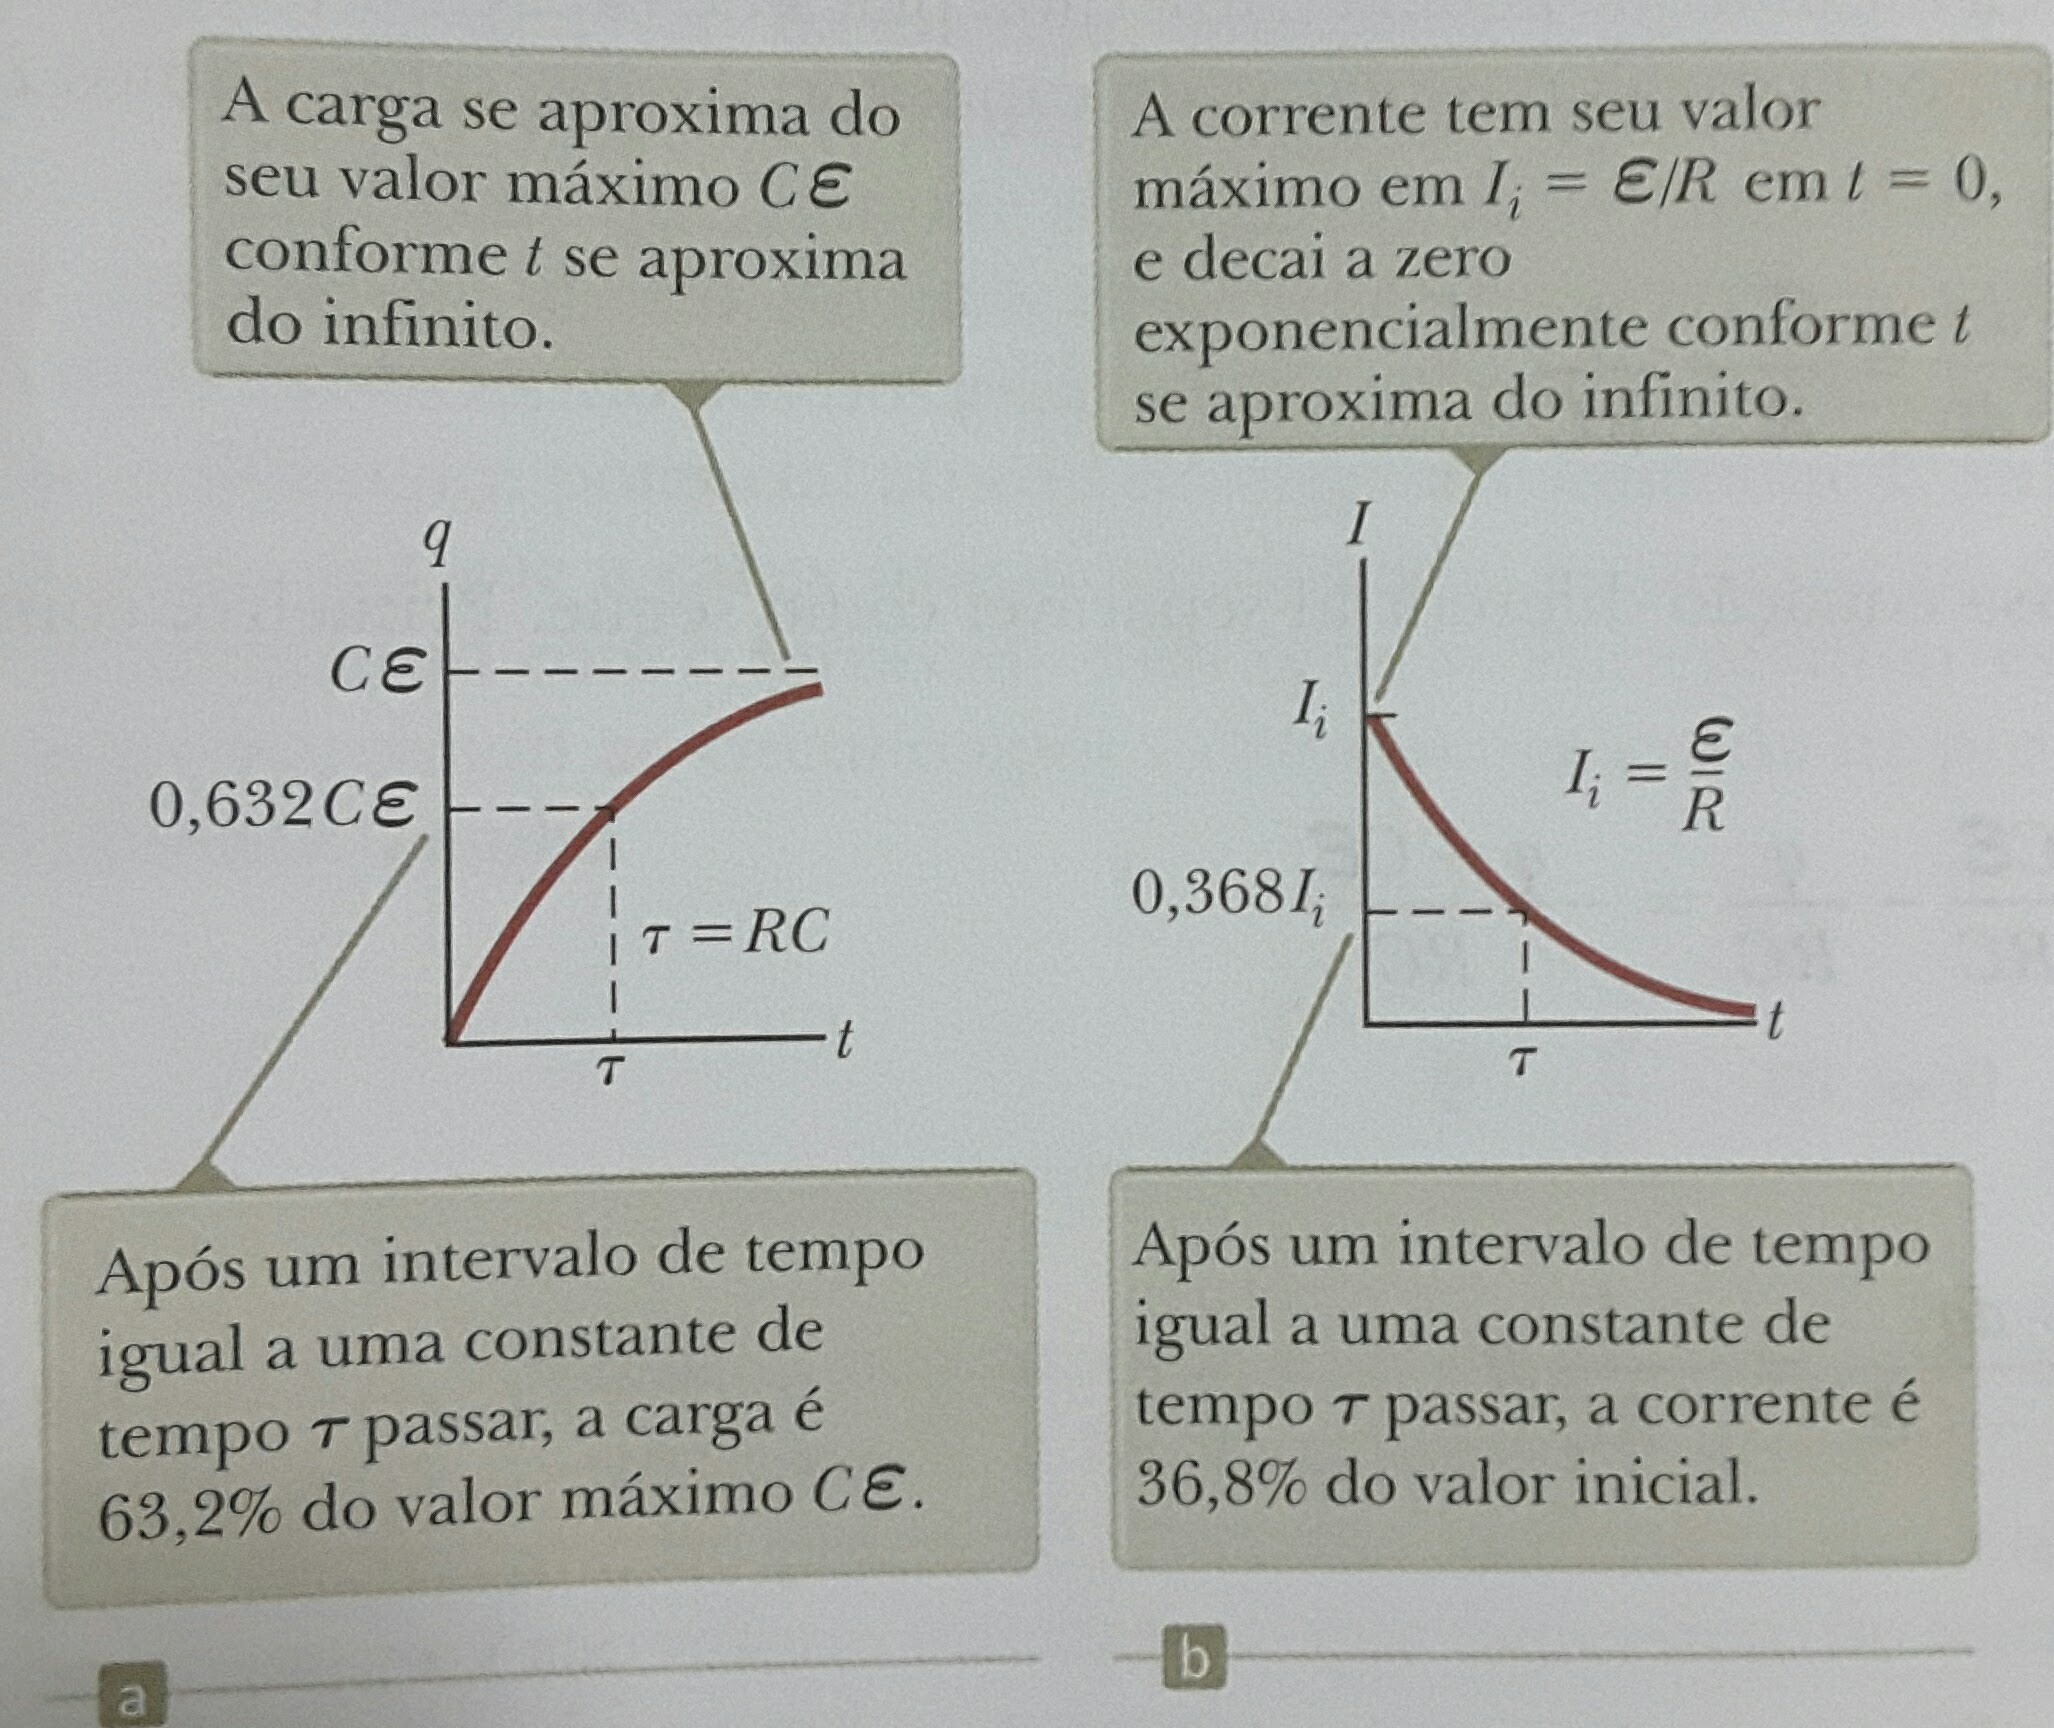
\includegraphics[width=15cm]{fig2}
\caption{(a) Representação de carga de carga de capacitor como função do tempo para o circuito mostrado na figura ativa \ref{fig:1}\textit{b}. (b) Representação de corrente como função do tempo para o circuito mostrado na Figura ativa \ref{fig:1}\textit{b}. \textit{Fonte: Jewett, JR Serway (2011)\cite{jeewett11}}}
\label{fig:2}
\end{figure}

Note que a carga representa é zero em $t=0$ e atinge o valor máximo $C\varepsilon$ em $t \to \infty$. A corrente tem seu valor máximo $I_i=\varepsilon / R$  em $t=0$, e decai exponencialmente a zero com $t \to \infty$. A quantidade $RC$, que aparece nos expoentes das Equações \ref{eq:4} e \ref{eq:5}, é chamada \textbf{constante de tempo} $\tau$ do circuito:

\begin{equation}\label{eq:6}
\tau = RC
\end{equation}

A constante de tempo representa o intervalo de tempo durante o qual a corrente diminui para $1/e$ de seu valor inicial; isto é, após o intervalo de de tempo $\tau$, a corrente diminui para $I=e^{-1}I_i = 0,368I_i$. após o intervalo de tempo 2$\tau$, a corrente diminui para \hbox{$I=e^{-2}I_i = 0,135I_i$,} e assim por diante. Do mesmo modo, em um intervalo de tempo $\tau$, a carga aumenta de zero para \hbox{$C\varepsilon[1-e^{-1}] = 0,632C\varepsilon$.}

A análise dimensional permite-nos ver que $\tau$ tm unidades de tempo:

$$
[\tau]=[RC]=\left[ \left( \frac{\Delta V}{I} \right) \left( \frac{Q}{\Delta V} \right) \right] = \left[ \frac{Q}{Q/\Delta t} \right] = [\Delta t] = T
$$

Como $\tau=RC$ tem unidades de tempo, a relação $t/RC$ é adimensional, já que deve ser o expoente de $e$ nas Equações \ref{eq:4} e \ref{eq:5}. A energia fornecida pela bateria durante o intrvalo de tempo necessário para carregar totalmente o capacitor é \hbox{$Q\varepsilon=C\varepsilon^2$.} Após o capacitor estar totalmente carregado, a energia nele armazenada é \hbox{$1/2 \, Q\varepsilon = 1/2\,C\varepsilon^2$,} que é somente metade\footnote{Sugestão de verificação desta afirmação mediante Problema 64 \cite{jeewett11}, que permite mostrar que a metade restante da energia fornecida aparece como energia interna no resistor.} da saída de energia da bateria.

\section*{Decarga do Capacitor}
 
Imagine que o capacitor na Figura Ativa \ref{fig:1}\textit{b} esteja completamente carregado. Há uma diferença de potencial $Q/C$ nele, e diferença de potencial \textbf{zero} no resitor porque $I=0$. Se a chave for colocada na posição \textbf{b} e $t=0$ \hbox{(Figura Ativa \ref{fig:1}\textbf{c}),} o capacitor começa a descarregar pelo resistor. Em algum tempo $t$ durante a descarga, a corrente no circuito é $I$ e a carga no capacitor é $q$. O circuito na Figura Ativa \hbox{\ref{fig:1}\textbf{c}} é o mesmo daquele na Figura Ativa \hbox{\ref{fig:1}\textbf{b},} exceto pela ausência de bateria (ddp da fonte). Portanto, eliminamos a força eletromotriz $\varepsilon$ da equação \ref{eq:1} para obter a equação de malha apropriada para o circuito na Figura Ativa \hbox{\ref{fig:1}\textbf{c}:}


\begin{equation} \label{eq:7}
- \frac{q}{C}-IR=0    
\end{equation}

Quando substituímos $I=dq/dt$ nesta expresão e re-arranjando os termos ela se torna

\begin{gather*}
    -R \frac{dq}{dt} = \frac{q}{C}\\
    \frac{dq}{q} = -\frac{1}{RC}dt
\end{gather*}

A integração desta expressão usando $q=Q$ em $t=0$ resulta

\begin{gather*}
    \int_{Q}^{q} \frac{dq}{q} = - \frac{1}{RC} \int_{0}^{t} dt\\
    ln\left( \frac{q}{Q} \right) = - \frac{t}{RC}
\end{gather*}

Multiplicando ambos os lados por $e$ e re-arranjando:

\begin{equation} \label{eq:8}
q(t) = Qe^{-t/RC}\;(\textbf{descarga do capacitor})
\end{equation}


A diferenciação da equação \ref{eq:8} com relação ao tempo resulta na corrente \textbf{instantânea} como função do tempo:

\begin{equation} \label{e:8}
I(t) = -\frac{Q}{RC}e^{-t/RC}\;(\textbf{corrente de descarga do capacitor})
\end{equation}

onde $Q/RC = I_i$ é a corrente inicial. \textbf{O sinal negativo indica que, conforme o capacitor descarrega, a direção da corrente é oposta a sua direção enquanto estava sendo carregado} (compare as direções de corrente nas Figuras Ativas \hbox{\ref{fig:1}\textit{b}} e \hbox{\ref{fig:1}\textit{c}).} Tanto a carga no capacitor quanto a corrente decaem exponencialmente a uma taxa caracterizada pela constante de tempo \hbox{$\tau = RC$.}

\vspace{5.0ex}
\hrule{}


 
\section{Experimento }

O circuito da figura 1 mostra um capacitor ligado em série com um resistor; este conjunto é conectado a um fonte de tensão constante (fonte DC).
\vspace{5.0ex} 

No instante em que se efetua o contato há um deslocamento de cargas no circuito de tal modo que a d.d.p. nas placas do capacitor tende a se igualar à d.d.p. da fonte. Haverá corrente no circuito apenas durante o tempo necessário para que esta igualdade seja verificada, e esta corrente tem valor máximo no momento em que o capacitor for ligado à fonte, caindo a zero após o capacitor estar completamente carregado. 

\vspace{5.0ex} 
É importante ressaltar que a corrente do circuito não se mantém constante porque à medida que as cargas vão se armazenando nas armaduras do capacitor, mais difícil se torna a nova entrada de cargas (repulsão elétrica), até que chega um momento em que não seja possível o armazenamento de novas cargas (uma vez que a tensão da fonte é fixa) e a corrente cai a zero. Neste momento, o capacitor inicialmente descarregado, atinge carga máxima.

 \vspace{5.0ex}
Deve-se ter o cuidado de não realizar tal experimento, carregando o capacitor, ligando diretamente na fonte, uma vez que não existe resistência elétrica R para limitar a corrente e ela tende ao infinito (se a resistência no gerador for baixa) , podendo, deste modo, danificar a fonte.

\vspace{5.0ex}

A carga adquirida pelo capacitor depende da voltagem aplicada aos seus terminais (havendo é claro, um limite, para que não haja danificação do dielétrico do condensador, o que ocorre quando sua “rigidez dielétrica” é ultrapassada. Para evitar danos no capacitor procure não ultrapassar o valor de tensão sugerido pelo fabricante, o que normalmente vem anotado no próprio corpo do capacitor. Esta tensão chama-se “tensão nominal”; normalmente um capacitor suporta um tensão superior à normal, entretanto, não é conveniente operar com tensões acima da normal.



 
\subsection{Material}
\begin{enumerate} 
\item { um capacitor eletrolítico na faixa (330-1000 $\mu F$) 16V }
\item {um resistor faixa (50- 180 $k\Omega$) }
\item { uma fonte DC na faixa (5-16V) - um cronômetro }
\item { uma chapinha de metal - cabos e jacarés }
\item {um multímetro }
\end{enumerate}

\subsection{Procedimento}

\begin{enumerate}  
    \item { Ligar a fonte em DC e regular para 5V }
    \item { Montar o circuito com o resistor e o capacitor conforme indica a figura 1. }
    \item {  Ligar o multímetro em paralelo ao capacitor e regular o mesmo para ler tensão em DC e na escala de até 20V. }
    \item { Anotar o tempo e a voltagem, nos terminais do capacitor, na hora de carregá-lo, em uma tabela a cada 10s; }
    \item { Prepare a tabela antes de começar a anotar os dados.  }
    \item { Antes de começar ou de ligar a fonte, verificar se está tudo certo:   }
    \begin{enumerate} 
        \item{O capacitor está esta ligado com a polaridade correta? (o terminal maior é o pólo positivo).  }
        \item{Quem vai controlar as anotações do tempo? }
        \item{Quem vai controlar as anotações dos valores de V (tensão)? }
    \end{enumerate}

\item{Desconecte o capacitor sem desligar a fonte (caso contrário o capacitor descarregará sobre a resistência interna da fonte). }
\item{Descarregue o capacitor na chapinha metálica (figura 2). }
\item{Faça os gráficos: $I\,x\,t$ e $Q\;x\;t$. }
\end{enumerate}

Figura 2 - Esquema de descarga de uma Capacitor sobre uma plaquinha metálica. 
 
\section{Relatório }
\begin{enumerate} 
    \item[$\bullet$]{ Descreva o experimento em detalhe. }
    \item[$\bullet$]{ Descreva a análise dos erros ou incertezas nas medidas. }
    \item[$\bullet$]{ Apresente os dados organizados em tabelas. }
    \item[$\bullet$]{ Apresente a análise dos dados e gráficos. }
    \item[$\bullet$]{ Apresente os resultados pedidos com todos os cálculos efetuados. }
\end{enumerate} 
\subsection{Questão}
\vspace{2.0ex}
Para enriquecer seu relatório:
\begin{enumerate} 
\item Depois de efetuar o experimento, você se acha capaz de fazer uma pesquisa bibliográfica buscando informações sobre onde e porquê se usam circuitos RC de Corrente contínua? 
\item Qual aimportância de se saber calcular o tempo de carga-descarga de um capacitor?
\end{enumerate}  
 
\begin{thebibliography}{9}

\bibitem{jifufrgs}
IF UFRGS - Instituto de Física - UFRGS
\emph{Circuitos Elétricos}, \\ <www.if.ufrgs.br/tex/fis142/mod07/m\_s02.html> - Acesso em 01/05/2017
 
\bibitem{jeewett11}
  JEWETT JR, J.W., SERWAY, R. A. 
  \emph{Física para cientistas e engenheiros: Eletricidade e magnetismo},
  CENGANGE Learning,
  São Paulo:
  2011

\bibitem{halliday3}
David Halliday, Robert Resnick, Jearl Walker; \emph{F Fundamentos de Física, Volume 3}, 8ª edição, São Paulo 2010. 
 
\bibitem{juraitis}
JURAITIS, K. R.; DOMICIANO, J. B.; \emph{Capítulo 1 - O Laboratório de Física - Introdução ao Laboratório de Física Experimental}, Londrina, PR, 2009
  
  
\end{thebibliography}

\newpage
\appendix

\section{\appendixname} \label{anx:a}
Regras para determinação das diferenças de potenciais pelo resistor e uma bateria (a bateria é assumida como não tendo resistência interna).

\begin{figure}[htp]
\centering
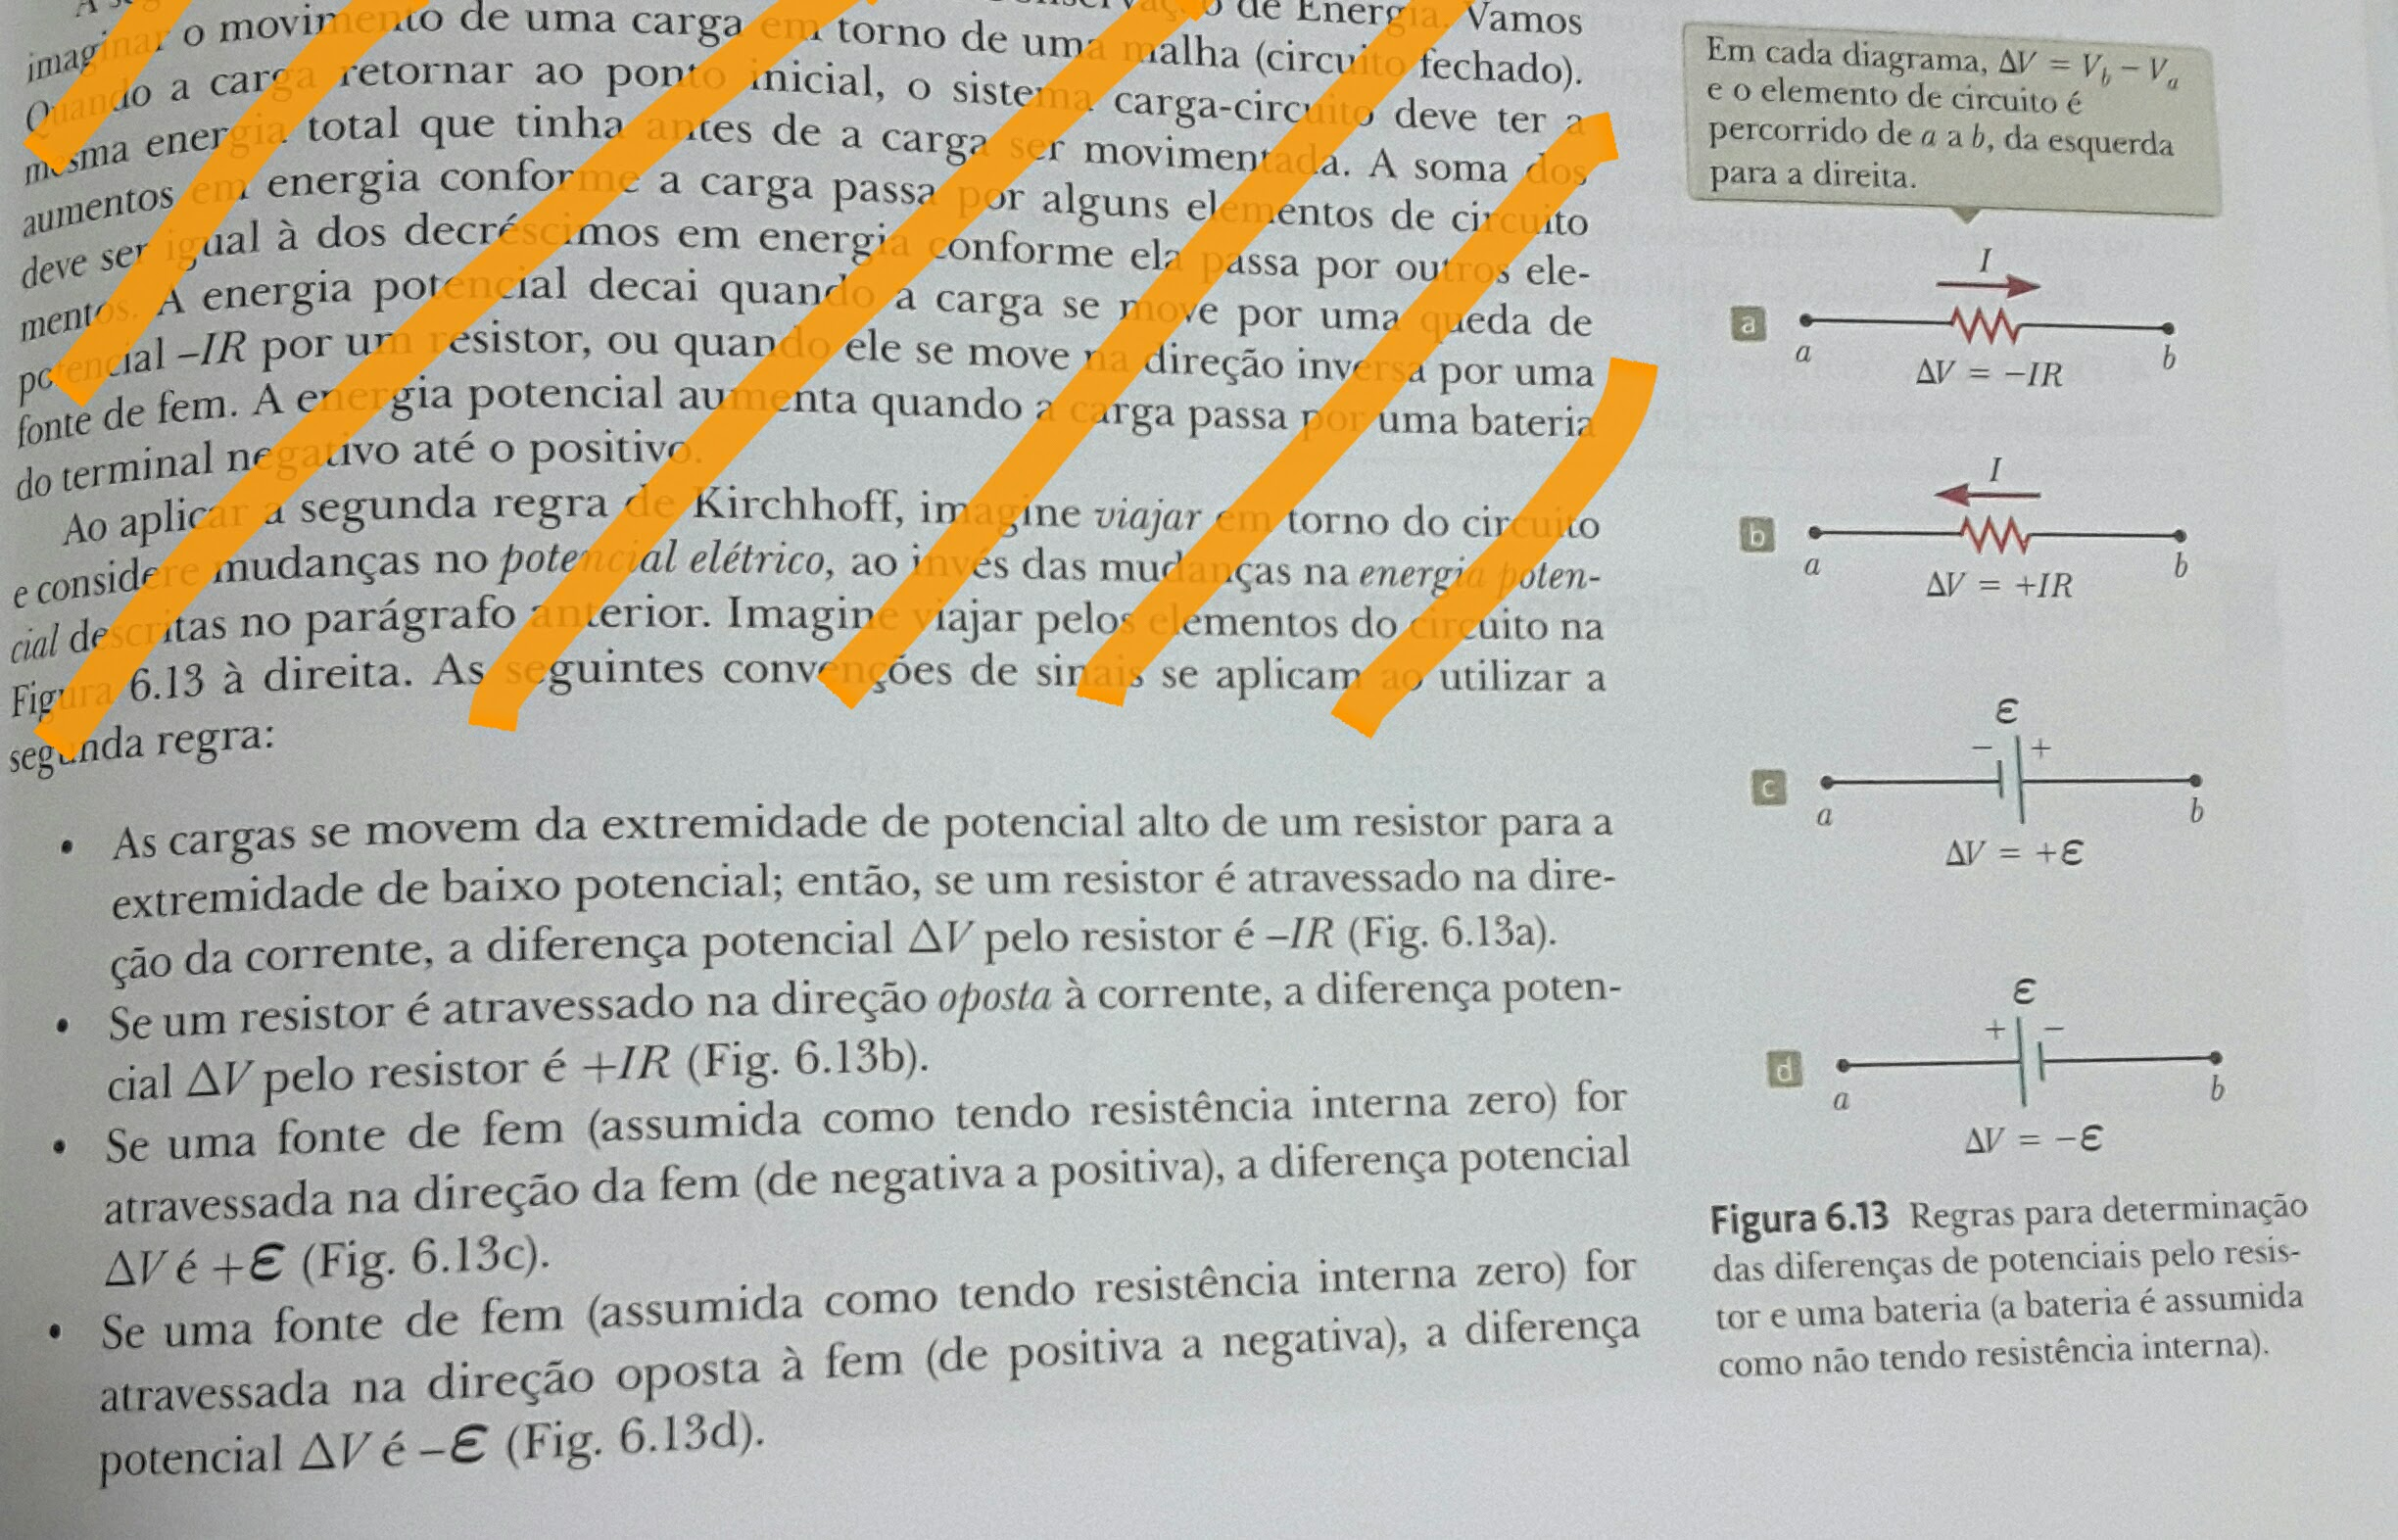
\includegraphics[width=16cm]{fig_ap}
\caption{Regras para determinação das diferenças de potenciais. \textit{Fonte: Jewett, JR Serway (2011)\cite{jeewett11}}}
\label{fig:lion}
\end{figure}

\end{document}